%======================================================================
\section{Condicionamento de sinais}\label{sec:condicionamento}
%======================================================================
Só um sensor do sistema entrega um sinal analógico: o LM35. Ele é o único que passa por
condicionamento eletrônico. Os outros entregam sinais digitais (PIR, portas, botão) ou já
digitalizados (MPU-6050), e o tratamento deles é feito no firmware, como filtro de
\textit{glitch}, \textit{debounce} e filtragem digital (Seção~\ref{sec:cond_digital}).

\subsection{Por que amplificar o LM35}

O ADC da ESP32-S3 tem 12 bits. Com a atenuação de 12\,dB, a única que cobre a saída do
amplificador, a faixa útil vai até cerca de 3,1\,V, ou seja, \adcLsb\,mV por contagem. O
LM35 entrega 10\,mV/°C: entre 0 e 57\,°C, sua saída ocupa só \lmOcupSemGanho\,\% da faixa do
ADC, e cada contagem vale \lmResolSemGanho\,°C (Figura~\ref{fig:faixa_adc}). Isso já atenderia
à resolução pedida (0,1\,°C) no papel, mas o ADC da ESP32 tem ruído e não linearidade de
várias contagens, e qualquer milivolt de ruído na trilha vira 0,1\,°C. Com um ganho de 5,5, o
sinal ocupa \lmOcupComGanho\,\% da faixa, cada contagem passa a valer \lmResolComGanho\,°C, e
o ruído que entra depois do amplificador pesa 5,5 vezes menos.

\begin{figure}[H]
\centering
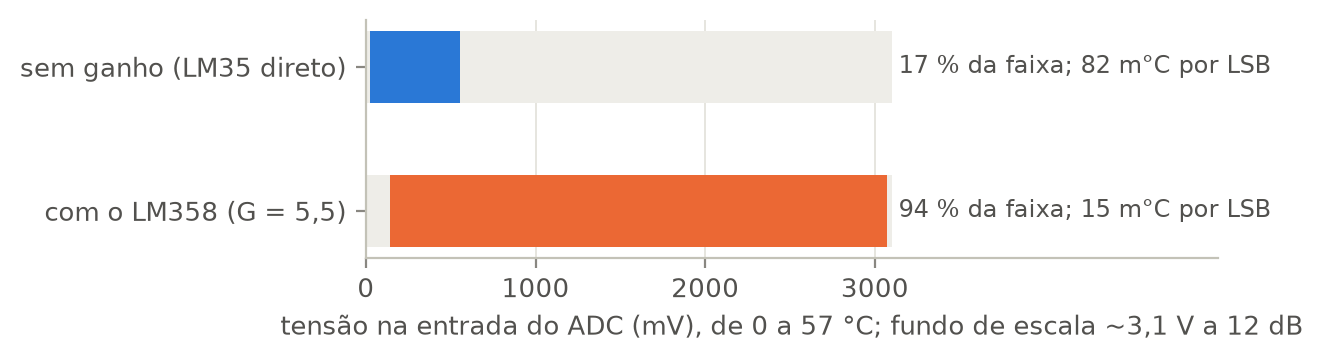
\includegraphics[width=\linewidth]{figuras/fig_lm35_faixa_adc.png}
\caption{Faixa do ADC ocupada pelo sinal de temperatura entre 0 e 57\,°C, sem e com o
amplificador, e o valor de uma contagem em °C.}
\label{fig:faixa_adc}
\end{figure}

\subsection{Circuito}

O condicionamento é um amplificador não inversor com o LM358 (Figura~\ref{fig:circuito_lm35}),
seguido de um filtro RC na entrada do ADC:
\begin{equation}
  G = 1 + \frac{R_2}{R_1} = 1 + \frac{9{,}1\,\text{k}\Omega}{2\,\text{k}\Omega} = 5{,}55 .
\end{equation}
O valor de projeto era 5,5, com $R_2 = 9$\,k$\Omega$; na série E24 o resistor mais próximo é
9,1\,k$\Omega$, compatível com o ganho medido no primeiro semestre (\lmGanhoMedido).

\begin{figure}[H]
\centering
\resizebox{0.95\linewidth}{!}{% Cadeia do LM35: sensor -> LM358 não inversor (G = 1 + R2/R1) -> filtro RC -> ADC.
\begin{circuitikz}[font=\footnotesize]
  % amplificador
  \draw (0,0) node[op amp, noinv input up] (OA) {\scriptsize U3A};
  \draw (OA.up) -- ++(0,0.5) node[above] {+5\,V};
  \draw (OA.down) -- ++(0,-0.35) node[ground] {};
  % realimentação
  \draw (OA.-) -- ++(-0.6,0) coordinate (nm);
  \draw (nm) -- ++(0,-1.4) coordinate (bot) to[R, l_={$R_2$ \SI{9.1}{\kilo\ohm}}] (bot -| OA.out) -- (OA.out);
  \draw (nm) -- ++(-1.3,0) coordinate (r1t) to[R, l_={$R_1$ \SI{2}{\kilo\ohm}}] ++(0,-2.2) node[ground] {};
  \draw (nm) node[circ] {};
  % sensor
  % na mesma altura da entrada + do amp-op, para o fio de V_out sair reto
  \node[draw, thick, minimum width=1.5cm, minimum height=1.3cm, align=center] (lm) at (OA.+ -| -5.4,0) {LM35DZ\\\scriptsize U2};
  \draw (lm.east) -- node[above, font=\scriptsize, pos=0.12] {$V_\text{out}$} (OA.+);
  \draw (lm.north) -- ++(0,0.55) coordinate (lmv) node[above] {+5\,V};
  \draw (lm.south) -- ++(0,-0.35) node[ground] {};
  \draw (lmv) ++(0,-0.25) -- ++(-1.1,0) coordinate (c1t) to[C, l_={$C_1$ \SI{100}{\nano\farad}}] ++(0,-1.9) node[ground] {};
  % saída: filtro RC e ADC
  \draw (OA.out) -- ++(0.5,0) coordinate (o) node[circ] {} to[R, l={$R_3$ \SI{10}{\kilo\ohm}}] ++(2.4,0) coordinate (g4)
        -- ++(1.0,0) node[right, align=left] {GPIO 4\\(ADC1\_CH3)};
  \draw (g4) node[circ] {} to[C, l={$C_3$ \SI{1}{\micro\farad}}] ++(0,-1.9) node[ground] {};
  \draw (o) -- ++(0,0.9) node[above, font=\scriptsize] {TP4};
\end{circuitikz}
}
\caption{Condicionamento do LM35 na PCB v1: amplificador não inversor (U3A, LM358) em
alimentação simples de 5\,V e filtro RC passa-baixa na entrada do ADC. Os capacitores de
desacoplamento ficam junto aos pinos de alimentação do LM35 (C1) e do LM358 (C2, omitido).
A outra metade do LM358 (U3B) é ligada como seguidor de 0\,V, para não oscilar.}
\label{fig:circuito_lm35}
\end{figure}

\paragraph{Alimentação simples.} No primeiro semestre, o LM358 era alimentado com $\pm$5\,V,
e o $-$5\,V vinha de um inversor na placa. Na PCB nova, ele é alimentado só com 5\,V e GND,
o que o datasheet permite (\textit{single supply}, 3 a 32\,V)~\cite{lm358}. Nessa condição,
a entrada aceita de 0 a $\sim$3,5\,V (o LM35 dá no máximo 0,6\,V) e a saída vai de
$\sim$20\,mV a $\sim$3,5\,V; o circuito usa de 0,14 a \lmVmaxCadeia\,V entre 0 e 57\,°C. Com
isso saíram da placa o inversor e suas peças, a fonte de ruído chaveada no bloco analógico e
o risco de tensão negativa num pino da ESP32.

\paragraph{Desacoplamento.} Um capacitor cerâmico de 100\,nF (X7R) junto ao pino de
alimentação do LM35 e outro junto ao do LM358, os dois ligados direto ao 5\,V da placa. Um
ramo de 5\,V separado para o analógico (ferrite ou 10\,$\Omega$ e 10\,µF) foi avaliado e
dispensado: o LM35 quase não sente o ruído da alimentação, o LM358 rejeita bem o ruído lento,
e o ruído rápido o filtro RC corta.

\subsection{Simulação e validação}\label{sec:validacao_lm358}

O circuito foi simulado em SPICE no primeiro semestre, com $G = 5{,}5$ ideal
(Figura~\ref{fig:spice}): a saída é uma reta de 0 a $\sim$3,3\,V para a entrada de 0 a 600\,mV.
Depois, ele foi montado em protoboard (Figura~\ref{fig:protoboard}) e medido junto com a
caracterização do sensor. A Tabela~\ref{tab:sim_bancada} compara a simulação e a bancada em
seis pontos da faixa.

\begin{figure}[H]
\centering
\begin{subfigure}[b]{0.49\linewidth}
  \centering
  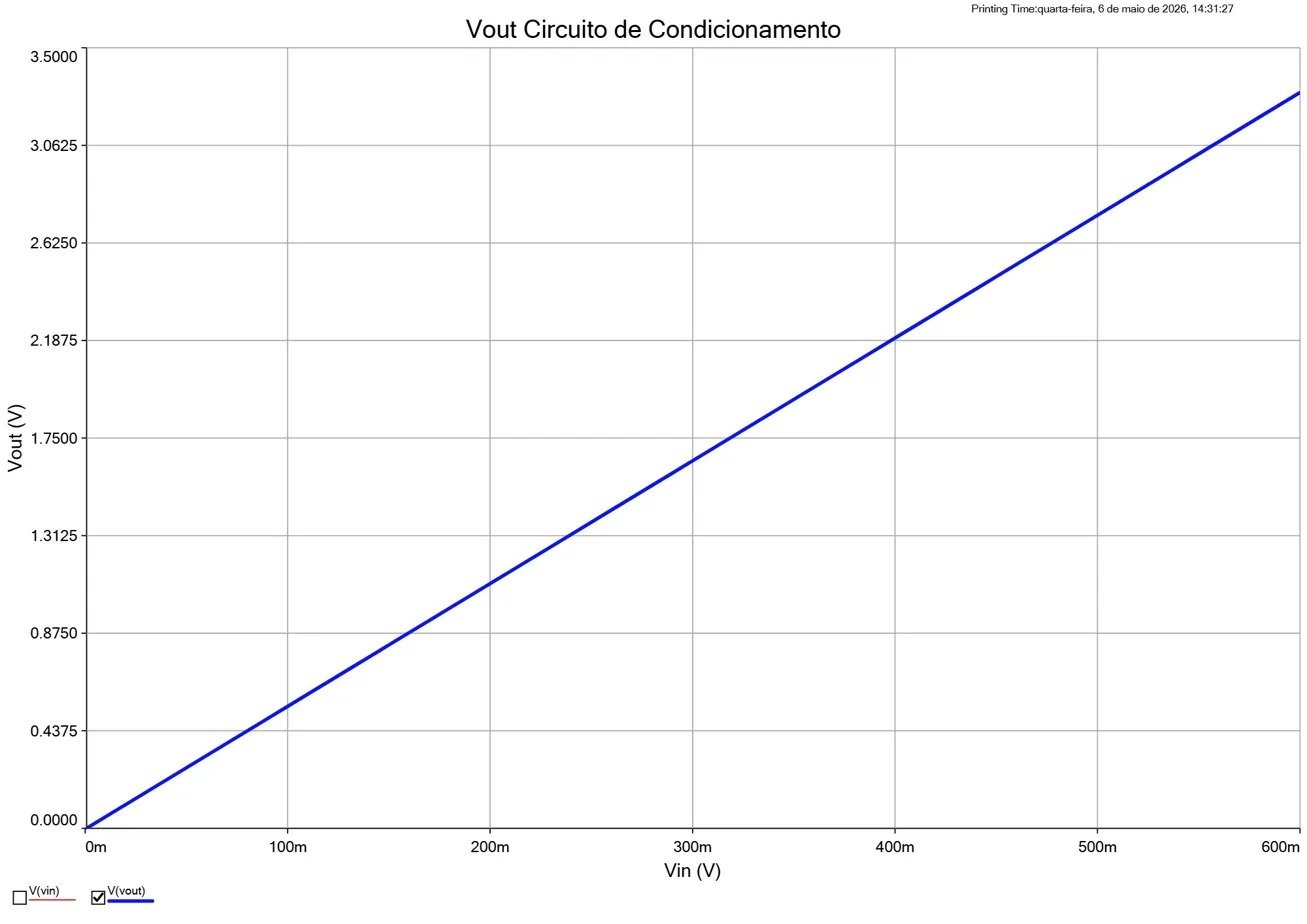
\includegraphics[width=\linewidth]{imagens/s1_spice_lm358.jpg}
  \caption{Simulação SPICE: $V_\text{out}$ em função de $V_\text{in}$.}
  \label{fig:spice}
\end{subfigure}\hfill
\begin{subfigure}[b]{0.49\linewidth}
  \centering
  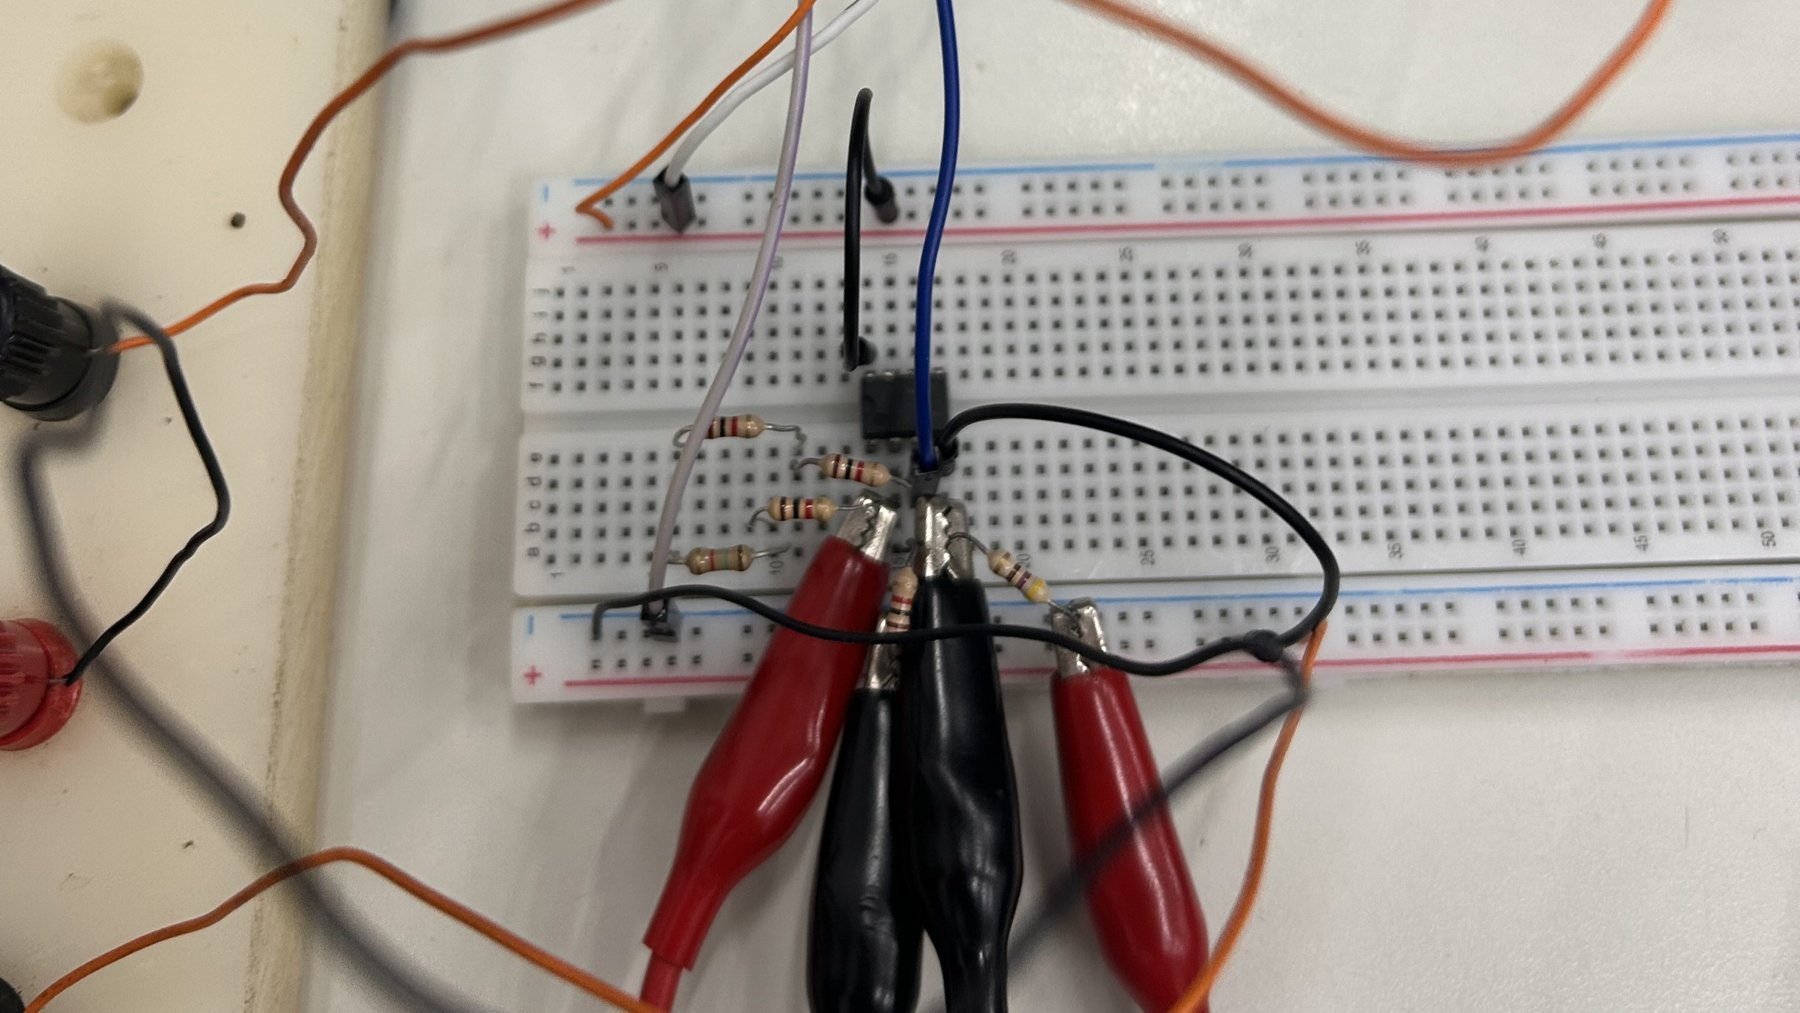
\includegraphics[width=\linewidth]{imagens/s1_protoboard_lm358.jpg}
  \caption{Montagem em protoboard.}
  \label{fig:protoboard}
\end{subfigure}
\caption{Validação do amplificador no primeiro semestre.}
\end{figure}

\begin{table}[H]
\centering
\caption{Saída prevista pela simulação ($G = 5{,}5$) e medida em bancada, para a mesma
entrada (dados do primeiro semestre).}
\label{tab:sim_bancada}
\small
\begin{tabular}{@{}S[table-format=2.1]S[table-format=3.2]S[table-format=4.2]S[table-format=4.1]S[table-format=+2.2]S[table-format=+1.2]@{}}
\toprule
{$T_\text{ref}$ (°C)} & {$V_\text{in}$ (mV)} & {$V_\text{sim}$ (mV)} & {$V_\text{med}$ (mV)} & {$\Delta$ (mV)} & {$\Delta/V_\text{med}$ (\%)} \\
\midrule
0,0  & 38,95  & 214,23  & 213,0  & -1,23  & -0,58 \\
9,0  & 108,80 & 598,40  & 602,2  & +3,80  & +0,63 \\
21,7 & 221,60 & 1218,80 & 1228,7 & +9,90  & +0,81 \\
33,3 & 332,10 & 1826,55 & 1843,6 & +17,05 & +0,93 \\
47,7 & 468,50 & 2576,75 & 2605,6 & +28,85 & +1,11 \\
62,2 & 603,60 & 3319,80 & 3354,5 & +34,70 & +1,03 \\
\bottomrule
\end{tabular}
\end{table}

O desvio cresce com a entrada e, em termos relativos, estabiliza perto de +1\,\%: é um erro
de ganho, não de \textit{offset}. O ganho real (\lmGanhoMedido) fica 1,1\,\% acima do ideal,
dentro da tolerância dos resistores. Como o firmware usa a curva medida da cadeia inteira
(Eq.~\ref{eq:cadeia}), esse erro não aparece na temperatura.

\subsection{Filtro RC na entrada do ADC}

Entre a saída do LM358 e o GPIO 4 há um resistor de 10\,k$\Omega$ em série e um capacitor
cerâmico de 1\,µF ao GND, colado no pino. É um passa-baixa de primeira ordem
(Figura~\ref{fig:rc_bode}):
\begin{equation}
  f_c = \frac{1}{2\pi R_3 C_3} = \frac{1}{2\pi \cdot 10\,\text{k}\Omega \cdot 1\,\mu\text{F}}
  \approx \rcFc\,\text{Hz}.
\end{equation}

\begin{itemize}
  \item Atenua \rcSessenta\,dB em 60\,Hz (a rede elétrica) e \rcMil\,dB em 1\,kHz, e fica abaixo
        do Nyquist das rajadas do firmware (amostras a cada 10\,ms, ou seja, 50\,Hz). A
        temperatura muda em minutos e passa inteira.
  \item Acomoda em $\sim$\rcAssentaMs\,ms ($5\tau$), muito menos que o intervalo de 60\,s entre
        medições.
  \item O capacitor fornece a carga que o capacitor de amostragem do ADC puxa a cada
        conversão, o papel do \textit{bypass} de 100\,nF recomendado pela documentação do
        ESP-IDF~\cite{espidf}.
  \item O resistor protege o pino: limita a corrente se a saída sair da faixa (ao ligar a
        placa, com o LM35 em mau contato, ou com uma ponta de prova no 5\,V). A queda nele é
        desprezível, porque só passa a corrente de fuga do pino, da ordem de nA.
  \item O capacitor é cerâmico (X7R): um eletrolítico tem fuga de µA, que nos 10\,k$\Omega$
        daria dezenas de mV de erro.
\end{itemize}

\begin{figure}[H]
\centering
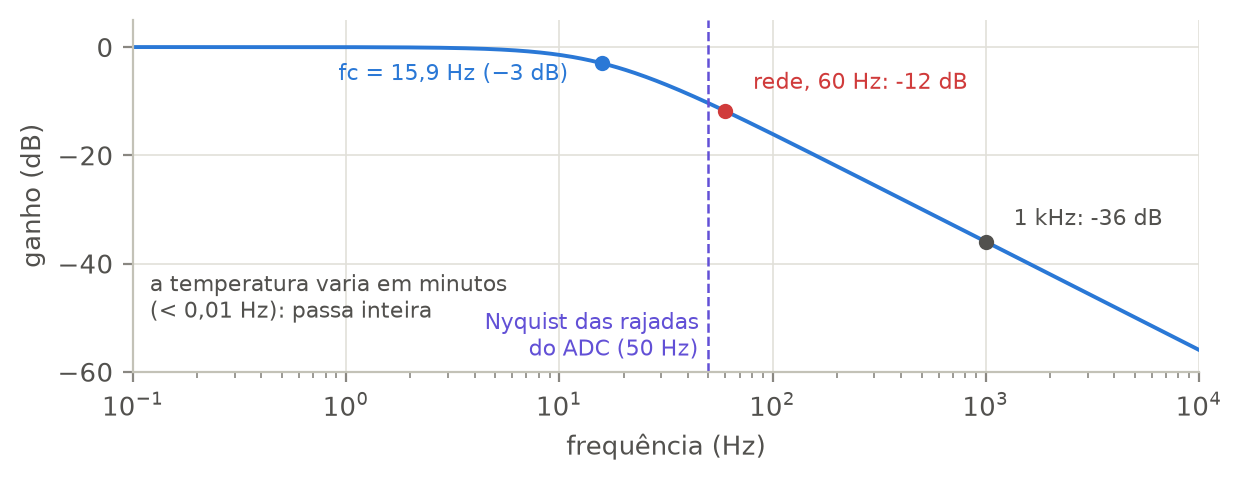
\includegraphics[width=\linewidth]{figuras/fig_rc_bode.png}
\caption{Resposta em frequência do filtro RC de 10\,k$\Omega$ e 1\,µF.}
\label{fig:rc_bode}
\end{figure}

\subsection{Aquisição da temperatura}

A cada 60\,s, a tarefa do LM35 faz 16 leituras do ADC1, canal 3 (GPIO 4), espaçadas de
10\,ms. Uma leitura por minuto basta: o ar do quarto leva dezenas de minutos para mudar, o
próprio LM35 leva minutos para acompanhá-lo, e a regra de temperatura espera 10\,min fora da
faixa. Toda leitura vai para a regra, mas só é publicada quando muda (Seção~\ref{sec:mqtt}). Cada leitura passa pela calibração do próprio chip (\code{adc\_cali}, que converte a
contagem em mV usando os parâmetros gravados de fábrica) e as 16 são promediadas, o que reduz
o ruído aleatório por um fator de $\sqrt{16} = 4$. A temperatura sai da curva da cadeia:
\begin{equation}
  T = \frac{V_\text{mV} - \lmBetaCadeia}{\lmAlfaCadeia} .
\end{equation}
Uma leitura fora de 0 a 57\,°C (o limite do ADC) é tratada como sensor solto: não é
publicada nem alimenta as regras, e o firmware avisa uma vez no log.

\subsection{Condicionamento digital dos outros sensores}\label{sec:cond_digital}

\paragraph{Portas e PIR.} Os dois são entradas digitais com interrupção nas duas bordas. Em
cada pino, o \textbf{filtro de \textit{glitch}} do GPIO da ESP32-S3 descarta pulsos mais curtos
que dois ciclos do relógio do IO-MUX: os picos captados pelos fios longos até a porta nem
chegam a gerar interrupção. O \textbf{\textit{debounce}} é por estabilização: a interrupção só
avisa que algo mudou, e a tarefa dos sensores lê o nível depois de 50\,ms sem nenhuma borda.
Assim, o repique do reed vira uma única transição, com o estado final. Na saída do PIR há um
resistor de 1\,k$\Omega$ em série (R4), que limita a corrente entre o módulo de 5\,V e o pino.

\paragraph{Botão.} \textit{Pull-up} interno, 100\,nF em paralelo e o filtro de
\textit{glitch}. O \textit{debounce} também é por estabilização, em 30\,ms: a interrupção pega
as duas bordas e só acorda a task do botão, que lê o nível quando a linha fica quieta. Um
bloqueio fixo depois de cada aperto, como os 300\,ms usados antes, engoliria o segundo toque
dos dois toques (Seção~\ref{sec:botao}).

\paragraph{MPU-6050.} O sinal inercial passa por dois filtros. O primeiro é o DLPF do próprio
sensor, em 44\,Hz, antes da decimação para 200\,Hz. O segundo é um passa-baixa Butterworth de
segunda ordem, em \bqFc\,Hz, aplicado aos 6 eixos na pulseira (Figura~\ref{fig:biquad}). Ele é um
\textit{biquad} da biblioteca ESP-DSP (\code{dsps\_biquad\_f32}), com os coeficientes
$\{b_0; b_1; b_2; a_1; a_2\} = \{\bqCoefs\}$, gerados pelo mesmo código Python que treina o
modelo de queda. Assim, o firmware filtra exatamente como o treino filtrou. Os movimentos do
corpo ficam abaixo de $\sim$12\,Hz e passam inteiros; o filtro tira o ruído e a vibração que
não ajudam a reconhecer uma queda.

\begin{figure}[H]
\centering
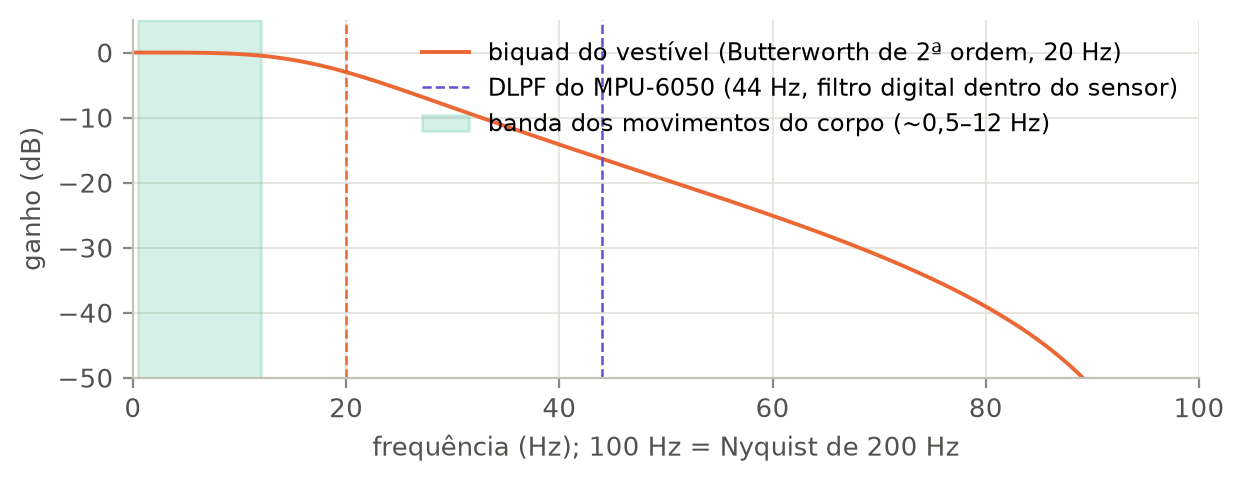
\includegraphics[width=\linewidth]{figuras/fig_biquad.png}
\caption{Resposta em frequência do passa-baixa de \bqFc\,Hz da pulseira ($f_s = \bqFs$\,Hz).}
\label{fig:biquad}
\end{figure}
